\chapter{Design}
This Chapter presents the scenario of this project, the goal of the system, and an overview of the actors and technical components. It also shows the methodology of the testing and gives an overview of the needed experiments.

\section{Scenario}
This project is designed for scenarios where artworks need to be transported securely from private collectors to museums. Throughout the journey, various stakeholders, including the collector, the museum, and insurers, are keen to ensure the safety of the artwork.
    
Before the transportation begins, the transporter sends the label, a unique identifier, to all involved parties, enabling them to track the artwork. Also before departure, predetermined thresholds for temperature and humidity are set. If these thresholds are breached during transit, stakeholders receive immediate alerts, allowing for fast intervention to reduce potential damage.

\begin{figure}[H]
    \centering
    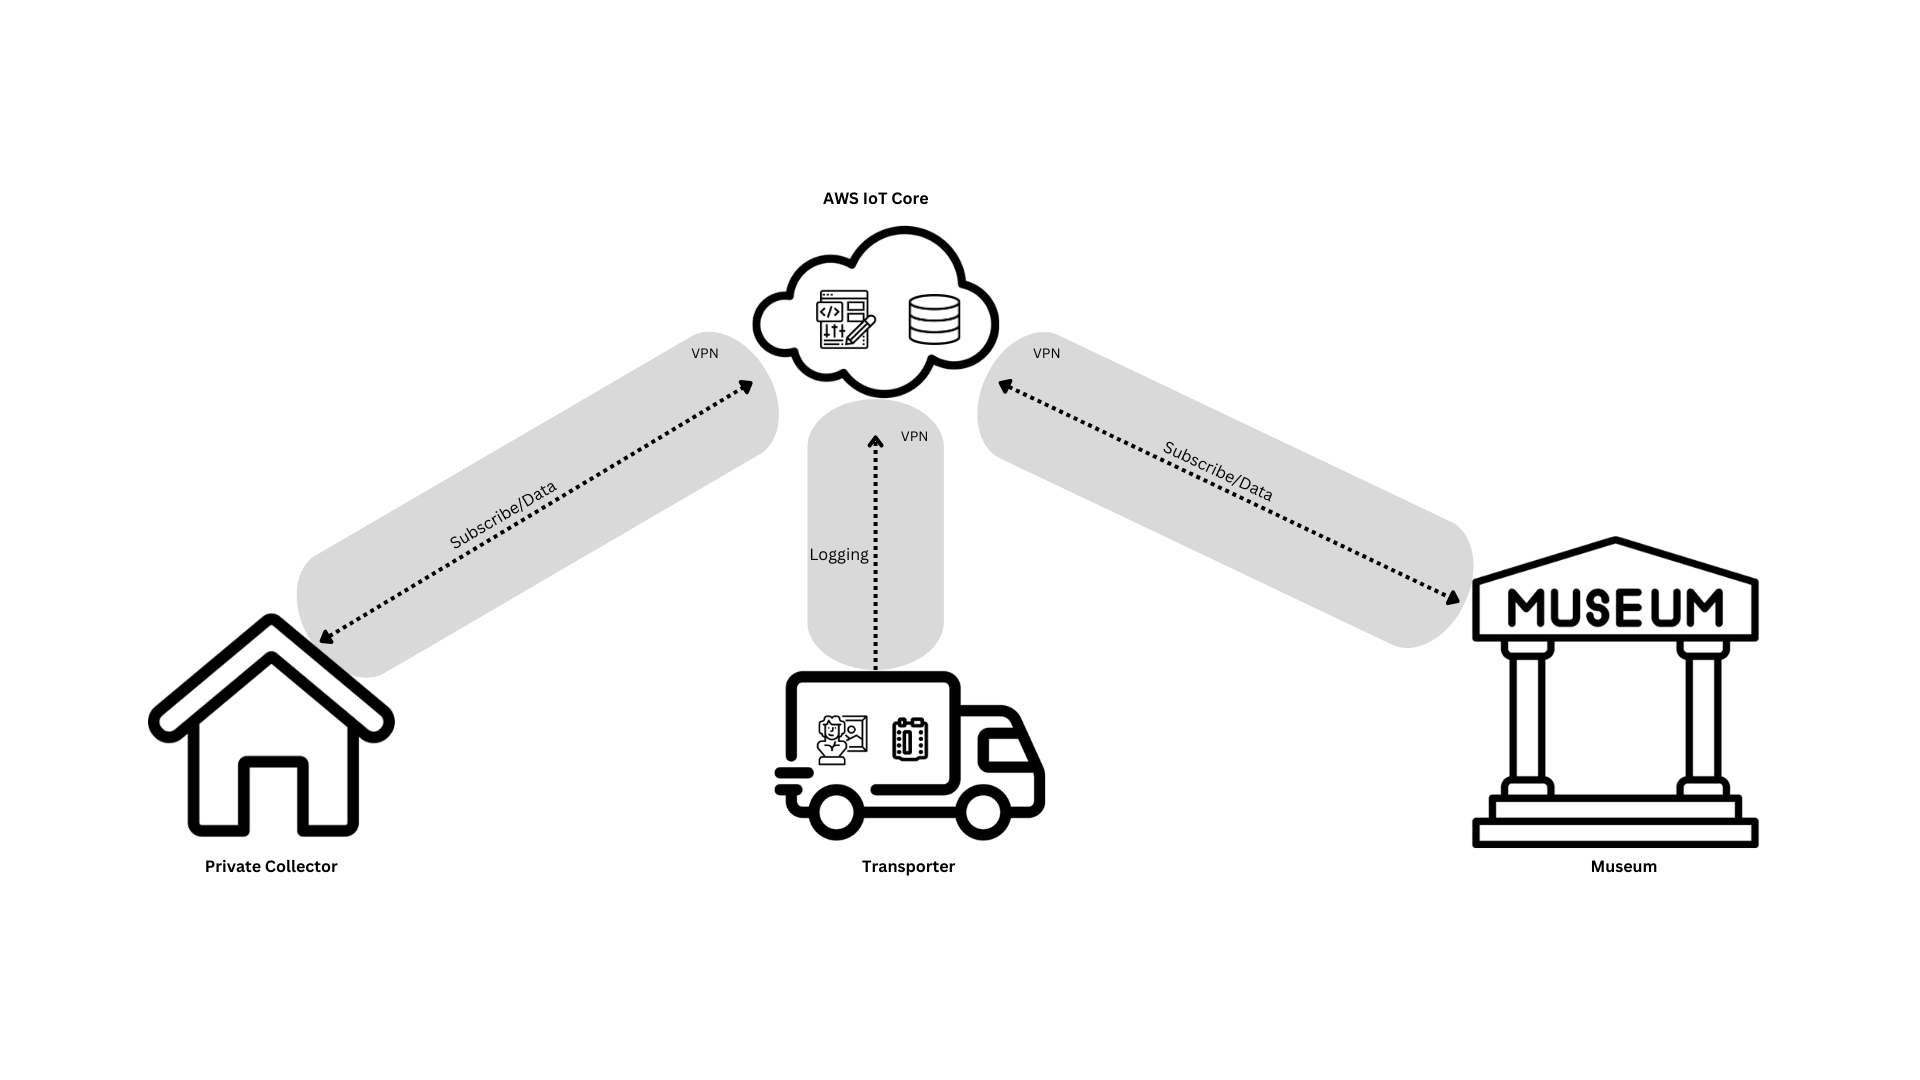
\includegraphics[width=\linewidth]{Scenario.png}
    \caption{Artwork Tracking Scenario}
    \label{fig:Artwork Tracking Scenario}
\end{figure}


\section{Goal}
The goal is to develop a monitoring system for the specified scenario.
The system includes a monitoring device, to capture temperature, humidity, and acceleration data. Utilizing an LTE connection, the device transmits this data along with a preassigned label to the cloud.
From there, the information is distributed to stakeholders, who are subscribed to the label, using the MQTT protocol.
To ensure the security and confidentiality of data transfer, VPN tunnels are implemented.

\section{Actors}
This system is designed for two actors, each defined as follows:
\begin{itemize}
    \item \textbf{Stakeholder:} The private collector, the museum, the insurer, or any other entity entrusted with the responsibility of monitoring the artwork during transportation.
    \item \textbf{Transporter:} A transportation company responsible for safely transporting the artwork from the private collector to the museum. They are also responsible for distributing the labels to the stakeholders and setting up the chosen thresholds.
\end{itemize}

\section{Technical Components}
The system consists of some technical components, that interact with each other and the actors to form a functional system. In Figure 4.2 the technical components and their connections are shown.

\textbf{IoT Device}

The monitoring device captures temperature, humidity, and acceleration data of the artwork throughout its transportation. Subsequently, it transmits the recorded data along with a corresponding label via an LTE connection to the cloud at regular intervals. Security measures are implemented through the utilization of a VPN.

\textbf{Cloud}

The cloud serves not only as a data storage for environmental data but also as a broker for the MQTT protocol. It receives data tagged with a specific label from the IoT device and forwards it to all subscribers of that label.

\textbf{Monitoring application}

To enable stakeholders to monitor the artwork effectively, a user interface is needed. This web application is specifically designed to ease the analysis of environmental data and promptly alert stakeholders when predefined thresholds are met.

\textbf{VPN}

VPN tunnels are implemented to secure the communication between the IoT device, the cloud, and the stakeholders. It reduces the risk of eavesdropping from third parties, by encrypting the data.


\section{Overview}
Figure 4.2 presents an overview of the system's architecture, illustrating the connections between various components and actors. It provides a visual representation of how each component interacts with others, offering insights into the system and the roles of different actors within it.

\begin{figure}[H]
    \centering
    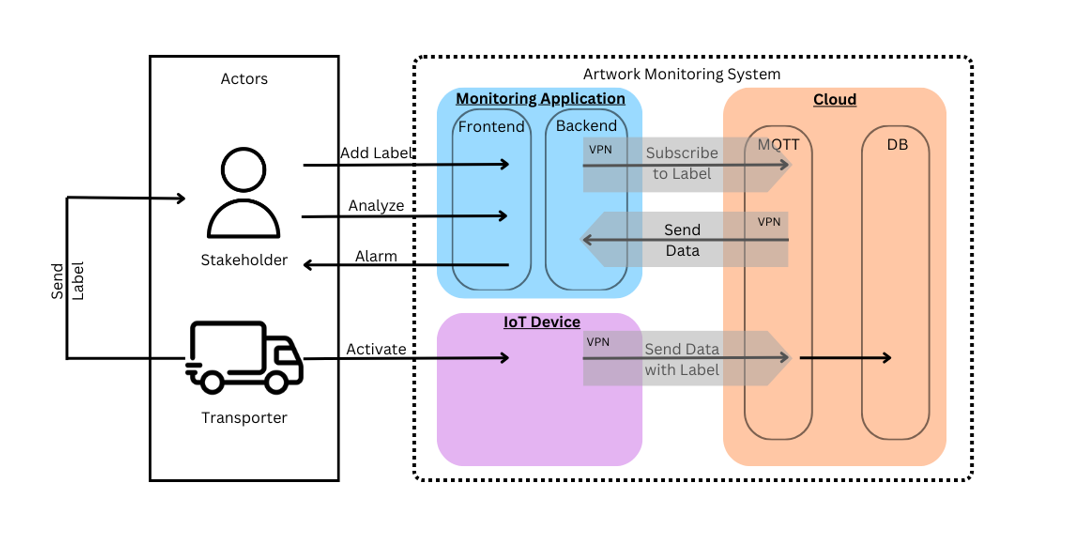
\includegraphics[width=1\linewidth]{System_Architecture.png}
    \caption{System Architecture}
    \label{fig:System Architecture}
\end{figure}

\section{Testing}
After implementing the system, thorough testing is essential. Therefore, three experiments are conducted. All experiments are initiated by adding the label to the monitoring application, for the stakeholder to be able to receive the data. At the end of each experiment, the transporter has to stop the data transfer by turning off the device and changing the label. This procedure ensures that stakeholders of the artwork do not have unauthorized access to data from future transports.

\textbf{Experiment 1}

In the first experiment, the label and thresholds are set on the IoT device, and the label is added to the monitoring application. Then the IoT device is placed in a backpack, and a walk is taken. Throughout the walk, the IoT device records the environmental data and sends them to the cloud. Meanwhile, at the starting point, a laptop assumes the role of a stakeholder, monitoring the artwork's condition by receiving real-time updates transmitted by the IoT device. As shown in Figure 4.3, the route spans 1.1 kilometers and is estimated to require approximately 15 minutes to walk. At the end of the walk, the device is turned off and the label is changed.

\begin{figure}[H]
    \centering
    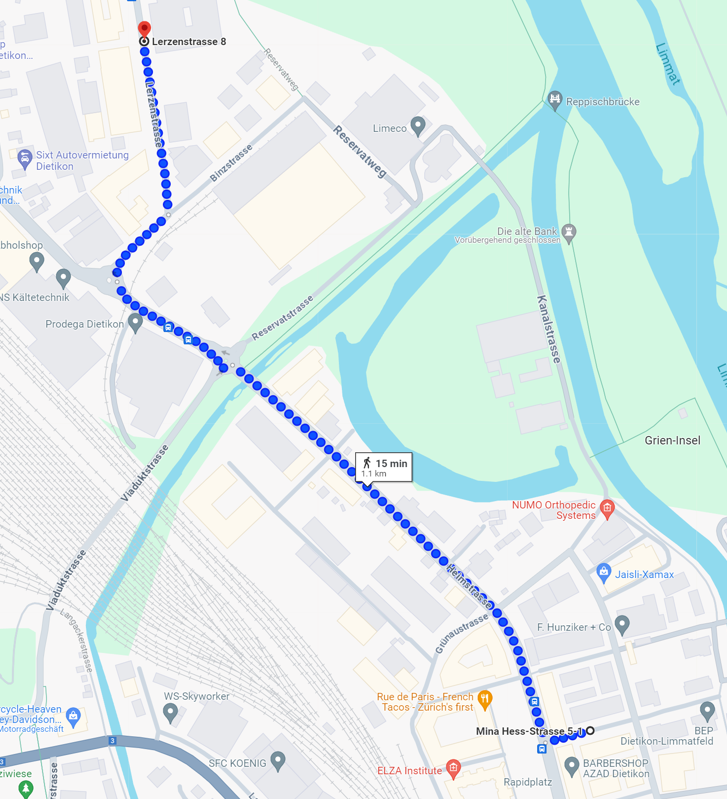
\includegraphics[width=0.4\linewidth]{Experiment_1_Route.png}
    \caption{Route Experiment 1}
    \label{fig:Route Experiment 1}
\end{figure}

\textbf{Experiment 2}

The second experiment involves a more dynamic setting, where the IoT device is installed within a car and gets transported, which makes it the closest to the use case. Before the transport begins, the label and thresholds are set on the IoT device, and the label is added to the monitoring application. During the ride, the IoT device continually captures temperature, humidity, and acceleration data and sends them to the cloud. Simultaneously, a laptop at the starting point works again as a stakeholder and monitors the condition of the artwork. As shown in Figure 4.4, the route spans 5.7 kilometers and is estimated to require approximately 8 to 10 minutes to drive. At the end of the transport, the device is turned off and the label is changed again.

\begin{figure}[H]
    \centering
    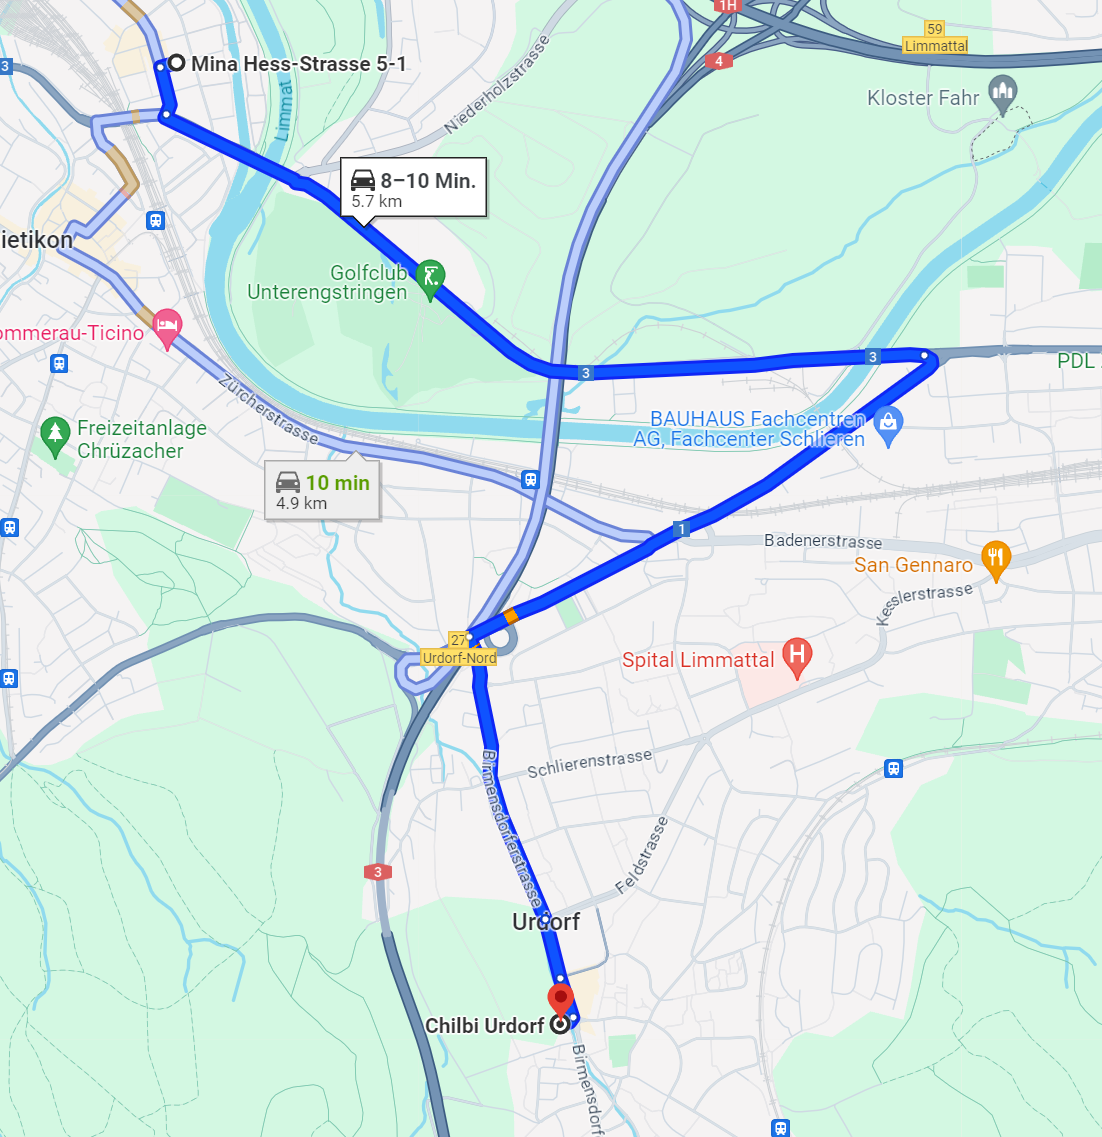
\includegraphics[width=0.5\linewidth]{Experiment_2_Route.png}
    \caption{Route Experiment 2}
    \label{fig:Route Experiment 2}
\end{figure}

\textbf{Experiment 3}

The third experiment introduces the IoT device to the potentially challenging environment of train travel, where the metallic structure of the train and other IoT devices within the train may present a risk of interference with data transmission. In this experiment, the IoT device gets transported on a train while monitoring it remotely from a laptop positioned at the starting point. As shown in Figure 4.5, the route is estimated to require approximately 36 minutes. In this experiment, the label and thresholds are also set at the beginning and the device is turned off at the end.

\begin{figure}[H]
    \centering
    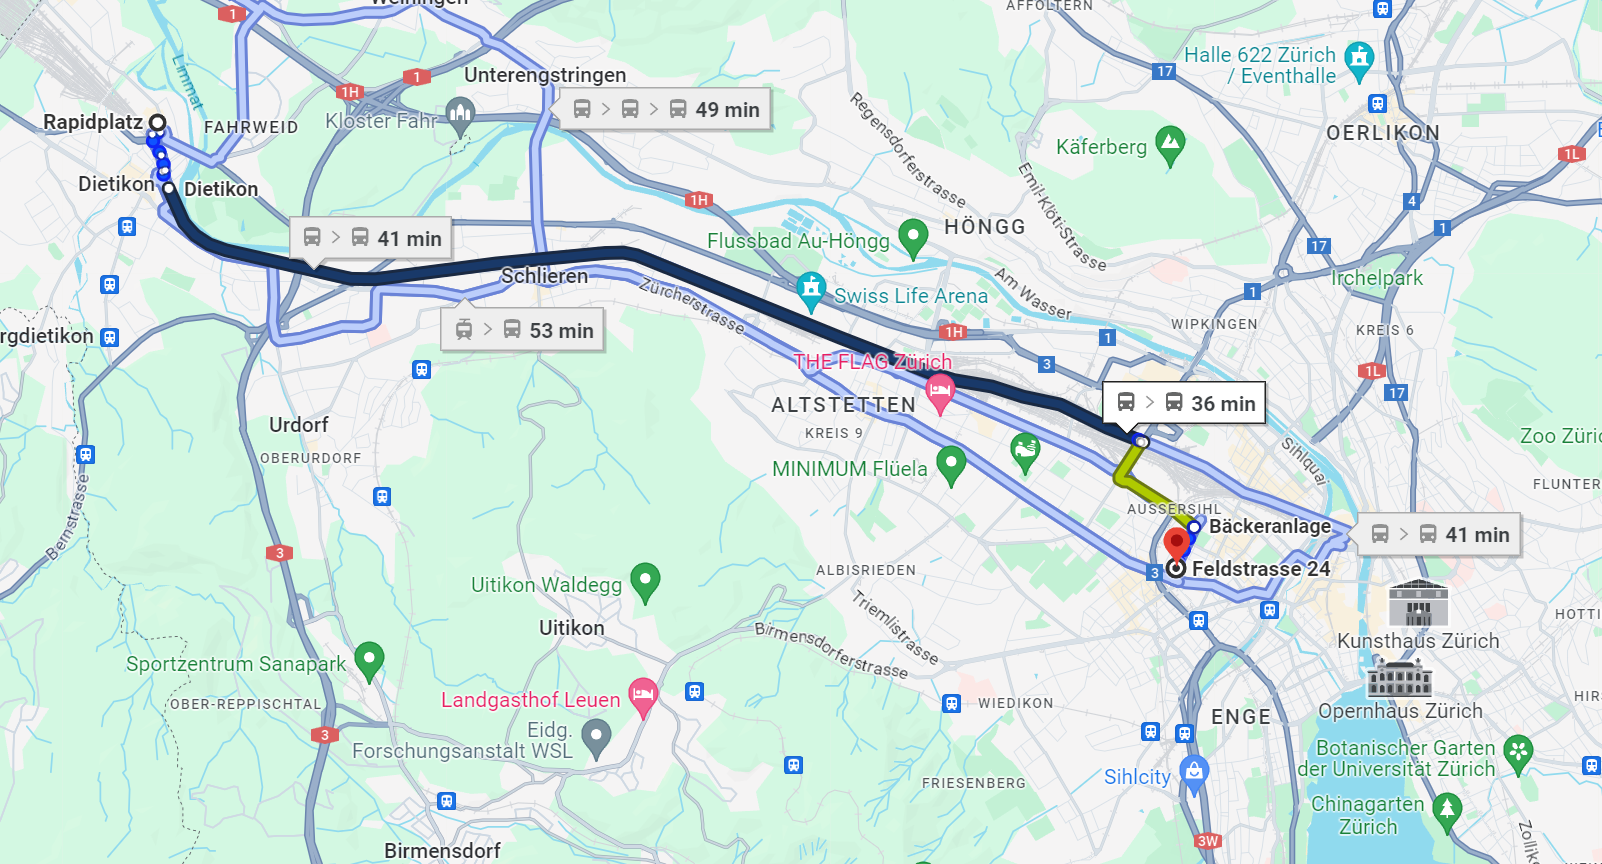
\includegraphics[width=\linewidth]{exp3_route.png}
    \caption{Route Experiment 3}
    \label{fig:Route Experiment 3}
\end{figure}

Table 4.1 gives us an overview of the different experiments.
It outlines which experiment assesses specific topics. All three experiments examine the connectivity, data measurement, and functionality in dynamic settings. Experiments 2 and 3 particularly focus on scenarios involving accelerated movement, while experiment 3 additionally investigates the resilience of the connection when the device is placed within a metal container.


\begin{table}[H]
    \centering
    \begin{tabular}{c|c|c|c|c|c}
         & Connection & Measurement & Dynamic & Speed & Container\\
         \hline
        Experiment 1 & $\surd$ & $\surd$ & $\surd$ & X & X\\
        \hline
        Experiment 2 & $\surd$ & $\surd$ & $\surd$ & $\surd$ & X\\
        \hline
        Experiment 3 & $\surd$ & $\surd$ & $\surd$ & $\surd$ & $\surd$\\
    \end{tabular}
    \caption{Experiments Overview Design}
    \label{tab:Experiments Overview Design}
\end{table}